\subsection{Equilibrium results}
\label{subsec:monte_carlo_results}
First, we study the relation between the order parameter~\eqref{eq:nematic_order_parameter} and $k_BT$ at equilibrium for different system densities. As we can see on the Figure~\ref{fig:op_kbt}, the nematic order increases with decrease of $k_BT$. The results are average over $200$ samples. Important to observer rapid increase in order parameter with the decay of thermal energy. The region of rapid increase shifts with densities, and for higher density the relation between order parameter and $k_BT$ closer to linear. As we can see, there is no systematic scaling with system size. In the section~\ref{sec:langevin_dynamics} we will discuss LD system relaxation towards the equilibrium results. Additionally important to note that the order parameter versus thermal energy dependency does not exhibit any criticality. The results are consistent with reported in literature (see~\cite{Marshall2015}). We must also note that statistical errors observed are of order $10^{-3}$.

\begin{figure}[h]
\centering
	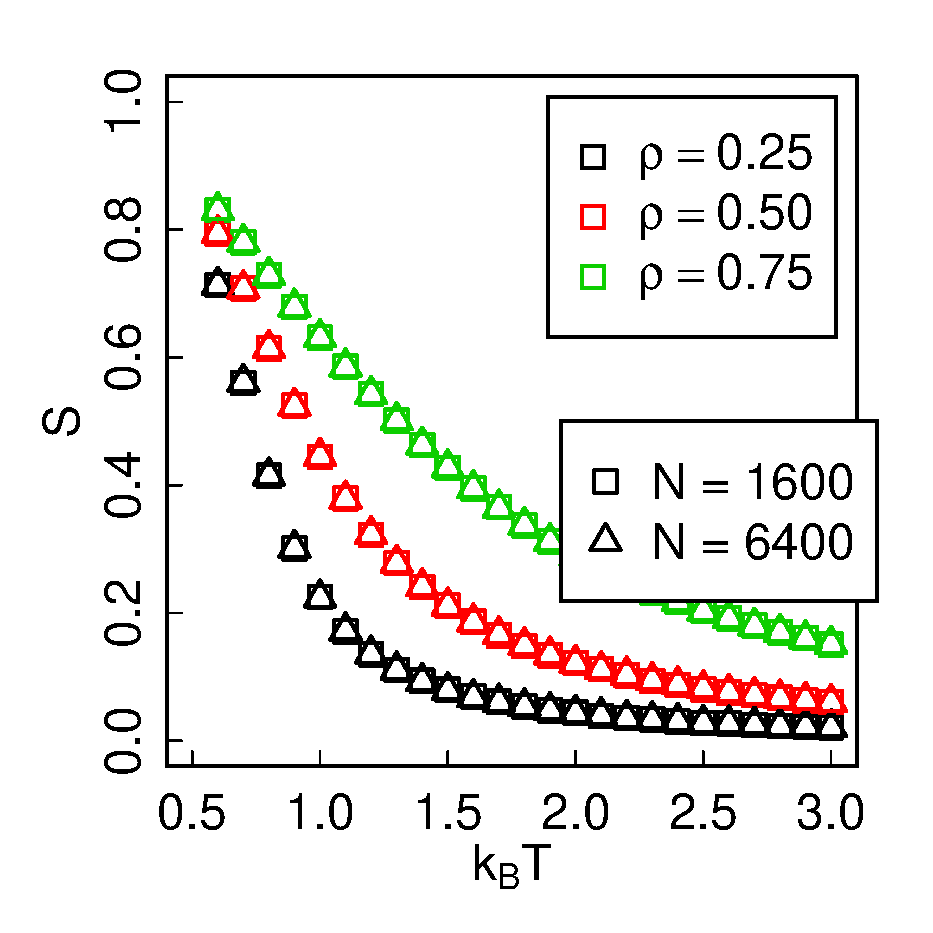
\includegraphics[width=0.5\textwidth]{Images/op_eq}
	\captionsetup{justification=centering, width=0.9\columnwidth}
	\caption{Order parameter defined by Eq.~\eqref{eq:nematic_order_parameter} versus $k_BT$ for Monte-Carlo simulations. Triangles shows results for $N = 6400$ and squares for $N = 1600$ particles. As we can see there is no systematic scaling with system size. The results are obtained by means of MC simulations, and are average over $200$ samples as described in sec.~\ref{subsec:simulation_details}}
	\label{fig:op_kbt}
\end{figure}

To characterize the dependence of the structure on $k_BT$, we analyze the orientation correlation (i.e. the level of co-alignment) of particles as function of distance between them. For all observed range of simulation parameters the correlation (i.e. co-alignment between dipole moments of two particles) decays exponentially with distance. For selected number of simulation parameters the results are presented at the Figure \ref{fig:dist_corr_eq}, done in log-linear scale. The dots are obtained with space sampling $\delta = 1/6$, and are averaged over $200$ samples with $N = 6400$ particles. Lines are obtained by linear approximation of the results in range $0.01 < C(\Delta z) < 0.45$.
\begin{figure}[h]
\centering
\begin{subfigure}[t]{0.32\textwidth}
	\centering
	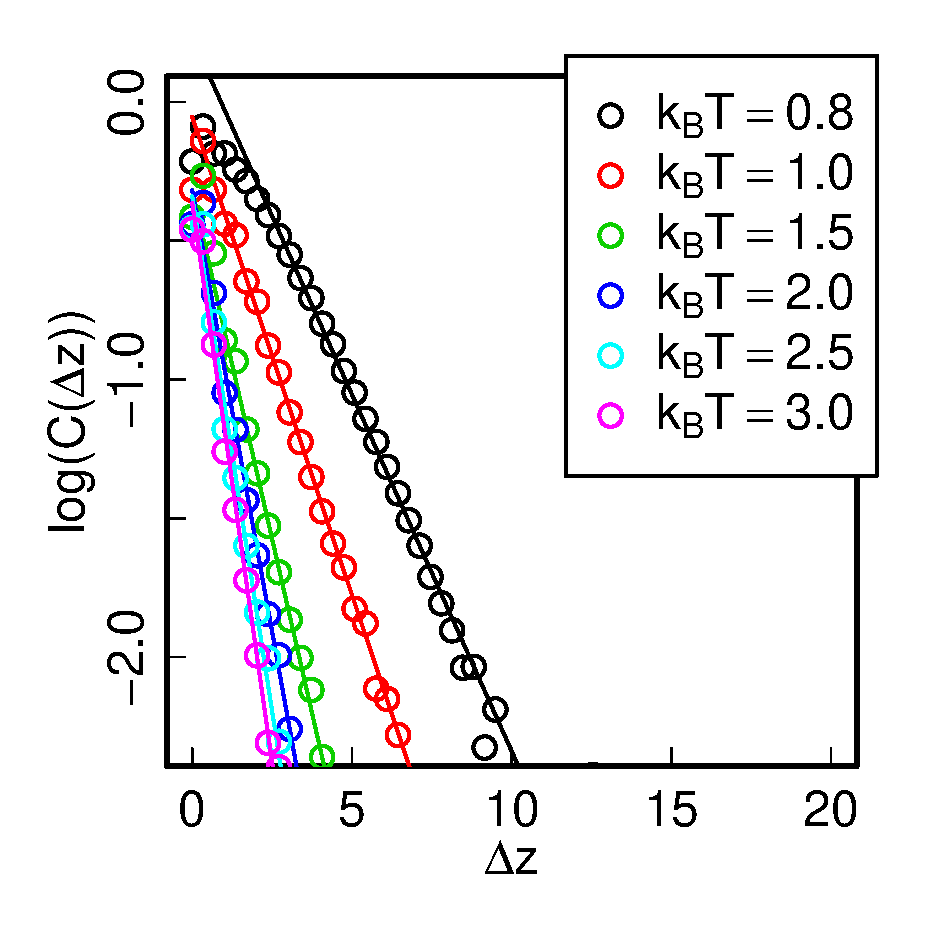
\includegraphics[width=\textwidth]{Images/distCor_25}
	\caption{$\rho = 0.25$}
\end{subfigure}
\begin{subfigure}[t]{0.32\textwidth}
	\centering
	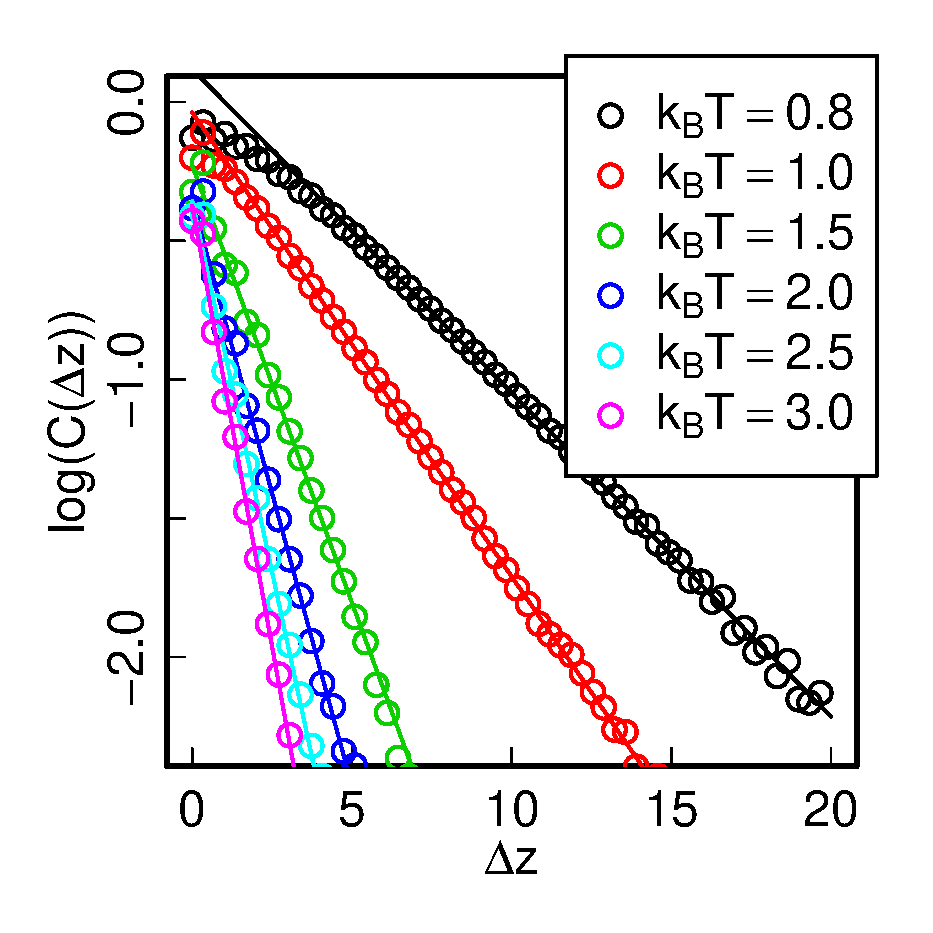
\includegraphics[width=\textwidth]{Images/distCor_50}
	\caption{$\rho = 0.50$}
\end{subfigure}
\begin{subfigure}[t]{0.32\textwidth}
	\centering
	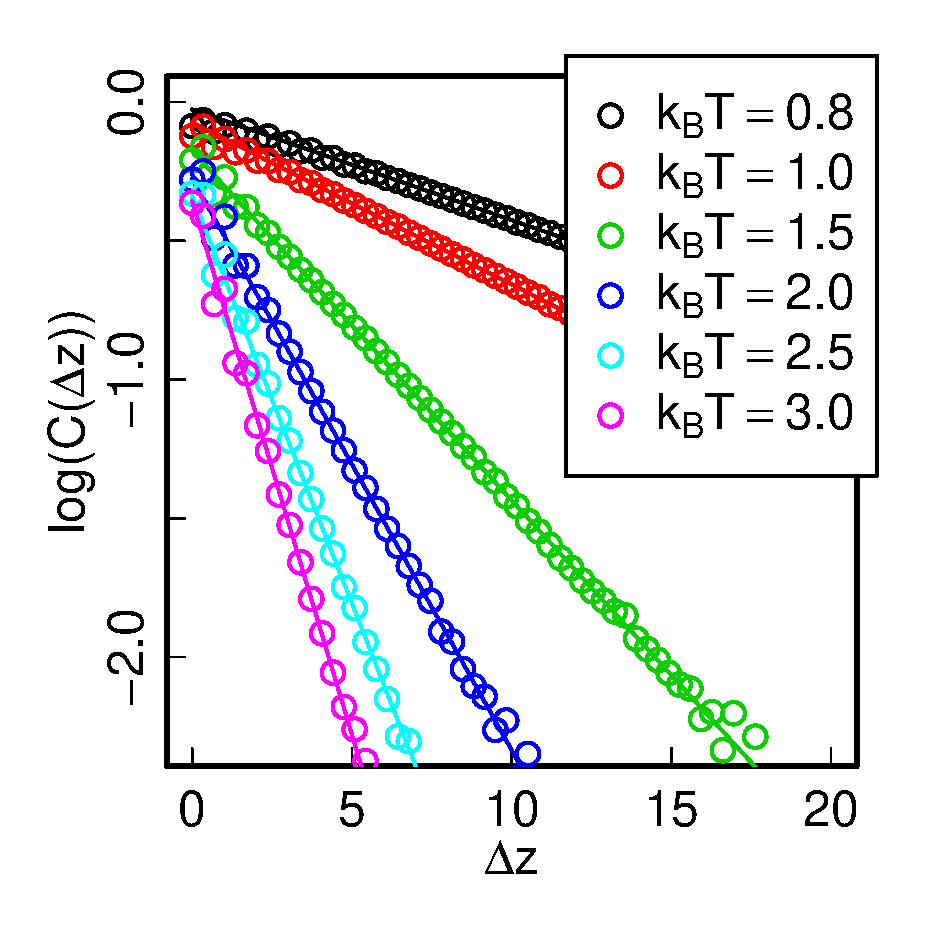
\includegraphics[width=\textwidth]{Images/distCor_75}
	\caption{$\rho = 0.75$}
\end{subfigure}
	\captionsetup{justification=centering, width=0.9\columnwidth}
	\caption{Orientation correlation as function of distance defined by Eq.~\eqref{eq:distance_correlation} for Monte-Carlo simulations in the log-linear scale. The points are calculated for simulations with $N = 6400$ particles and the results are averaged over $200$ samples as described in sec.~\ref{subsec:simulation_details}. Lines are obtained by linear approximation of the results in range $0.01 < C(\Delta z) < 0.45$.}
	\label{fig:dist_corr_eq}
\end{figure}

The exponential decay of correlation with length for every combination of simulation parameters shows that we do not have any critical transition occurring in the system under study, despite non-zero order parameter observed above.

We could now write $C(\Delta z)$ as
\begin{equation}
	\label{eq:slopes_def}
	C(\Delta z) \propto \exp\left[-\frac{\Delta z}{r^*(k_BT, \rho)} \right]
\end{equation}
where $r^*$ is the correlation length and depends on the system density and $k_BT$. The dependence of $r^*$ on the $k_BT$ for different system densities is shown at the Figure \ref{fig:dist_corr_eq_slopes}. We must note the similarity in behaviour of order parameter and the correlation distance. Additionally, the correlation distance never approaches the infinity for non-zero $k_BT$. \textcolor{red}{The relation is likely power law, do I need to mention this and add picture?}

\begin{figure}[h]
\centering
\begin{subfigure}[t]{0.5\textwidth}
	\centering
	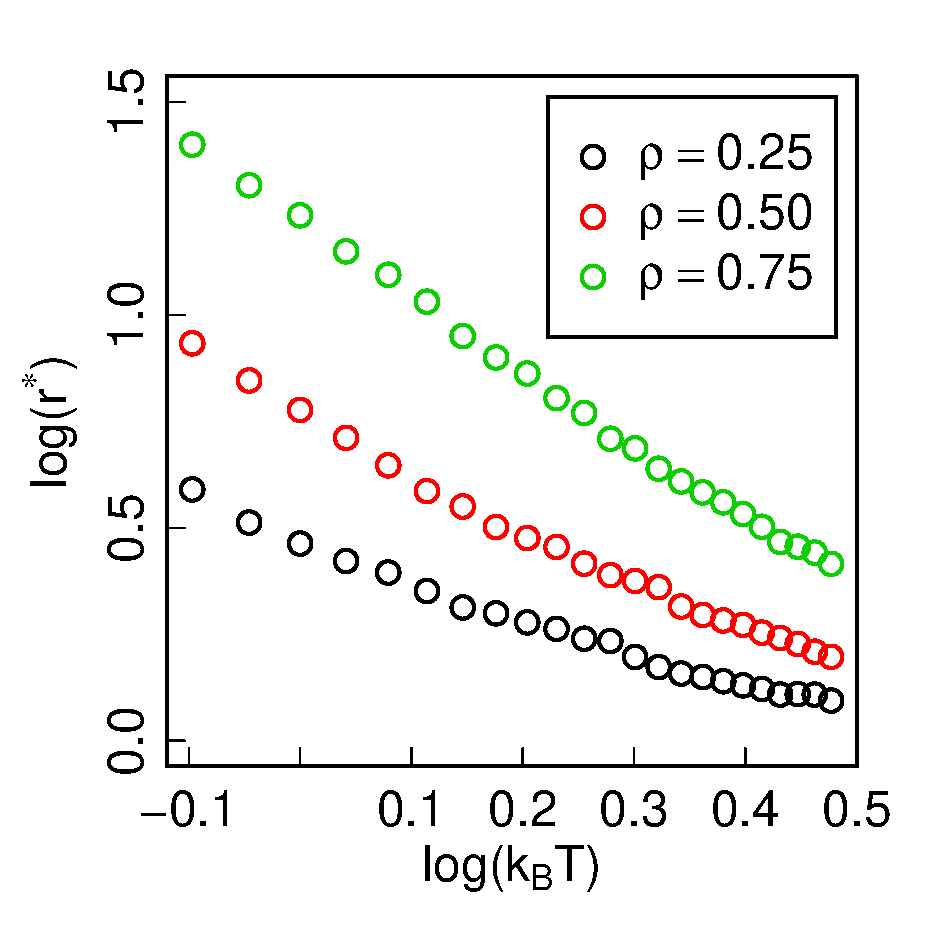
\includegraphics[width=\textwidth]{Images/correlation_length_eq}
\end{subfigure}
	\captionsetup{justification=centering, width=0.9\columnwidth}
	\caption{$r^*$ as defined in \eqref{eq:slopes_def}, obtained as inverse slope of orientation correlation shown at Figure~\ref{fig:dist_corr_eq}.}
	\label{fig:dist_corr_eq_slopes}
\end{figure}

% Defining ``chain'' we can distinguish three cases for the separation distance $d$. First being $d \ll R$ where $R$ is particle radius. That way we effectively treat all particles as ``unchained''. Second case is when $D \leq d < 2 D$, in which the ``chained'' particles form a compact cluster. And the third case is $d \sim L$, where $L$ is system size, in which the ``chain'' breaks only if particles orientations are not co-aligned with $z$ axis and each other.